\section{Dassault Mirage III}

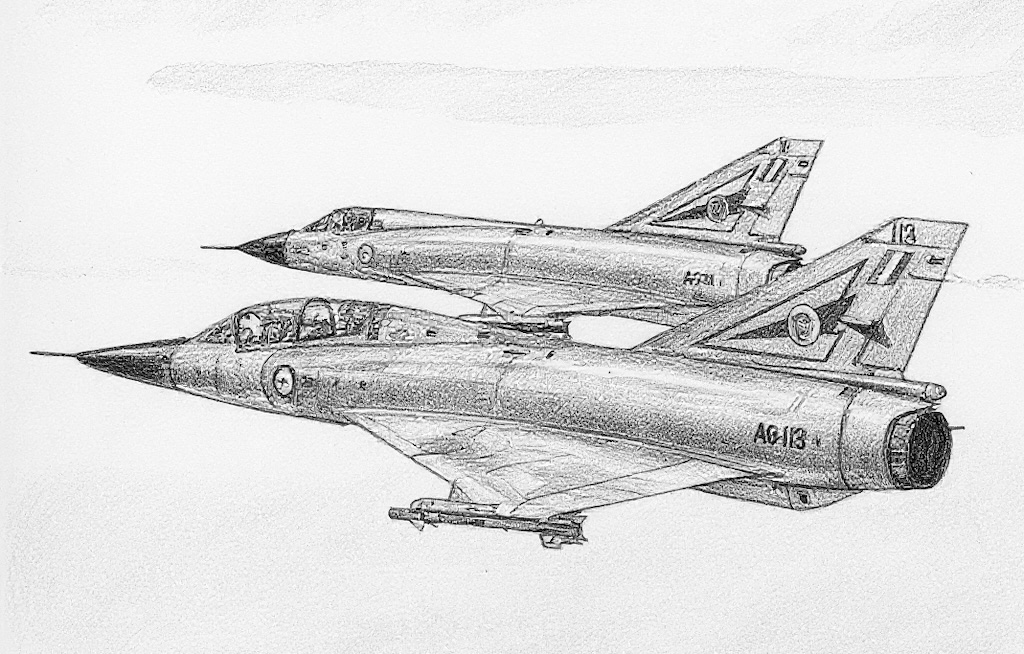
\includegraphics[width=\linewidth]{Mirage III.jpg}

The Dassault Mirage III is a supersonic interceptor and multirole aircraft.
\note{Sources}{
    \begin{itemize}
        \item Goebel, \href{https://airvectors.net/avmir3.html}{Air Vectors} (\href{https://web.archive.org/web/20260323015359/https://airvectors.net/avmir3.html}{Wayback})
        \item Kettle, “South Atlantic War”, Clash of Arms Games, 2nd Edition, 2002.
        \item Reid, “\href{https://artmandelta.com/wp-content/uploads/2024/10/Mirage-III-in-SAAF-Service-Part-9-by-Malcolm-Reid.pdf}{South African Air Force Mirage III and Cheetah: External fuel tanks},” October 2023 (Revision 0)
        \item \href{https://en.wikipedia.org/wiki/Dassault_Mirage_III}{Wikipedia on the Mirage III}
        \item \href{https://en.wikipedia.org/wiki/DEFA_cannon}{Wikipedia on the DEFA cannon}
        \item \href{https://en.wikipedia.org/wiki/R.530}{Wikipedia on the R.530}
        \item \href{https://en.wikipedia.org/wiki/R.550_Magic}{Wikipedia on the R.550}
        \item \href{https://en.wikipedia.org/wiki/Martel_(missile)}{Wikipedia on the Martel}

    \end{itemize}
    \noteparagraph{Photo Credit}
    \begin{itemize}
        \item \href{https://commons.wikimedia.org/wiki/File:Two_Mirage_III_of_the_Royal_Australian_Air_Force_1.JPEG}{Curt Eddings} (Public Domain)
    \end{itemize}
}

\subsection{Versions}

\subsubsection{Mirage IIIE}

The IIIE has an improved Cyrano-II radar, an extended fuselage to give room for more fuel and improved avionics including a RWR, and a slightly more powerful Atar 09C-3 engine.%
\note{IIIEA ADC}{
    The ADC is based on those in {\APJ} 20 and 44.

    \noteparagraph{RWR}
    Goebel states the E gained an RWR. I assume RWR-A.

    \noteparagraph{Station Limits}
    The station limits on the earlier ADCs need revision. The Mirage III can carry the TK-500 MRT, JL-100/JL-500 RPTs, of 1700L FTs on the inner-wing station and 1300L FTs on the centerline station (Kettle and Reid). In {\AirStr}, the TK-500 MRT has a weight of 1100~lb and can carry up to 2200~lb of bombs, for a total of 3300~lb, and the JL-100/JL-500 RPTs have a weight of 900/3000~lb. The 1300L FT from the IIIS weights 2540~lb and the 1700L FT from the IIIS in {\APJ}~39 weighs 3340~lb.

    The ADC for the IIIE in {\APJ} 20 has:
    \begin{itemize}[nosep]
        \item centerline: 1800 lb
        \item inner wing: 3000 lb
        \item outer wing: 550 lb
    \end{itemize}
    The ADC for the IIIE in {\APJ} 44 has:
    \begin{itemize}[nosep]
        \item centerline: 2600 lb
        \item inner wing: 1850 lb
        \item outer wing: 370 lb
    \end{itemize}
    The ADC for the IIIS in {\APJ} 39 has:
    \begin{itemize}[nosep]
        \item centerline: 2550 lb
        \item inner wing: 260 lb (for Falcons)
        \item inner wing: 1230 lb but can be overloaded to 2540 lb for 1300L FT (limited to HT) or 3340 lb for 1700L FT (limited to TT).
        \item outer wing: 370 lb
    \end{itemize}
    Kettle has these limits for the IIIEA (and also for the Dagger):
    \begin{itemize}[nosep]
        \item centerline: 1180 kg = 2600 lb
        \item inner wing: 840 kg = 1850 lb, but capable of carrying 1300L FT (2540 lb)
        \item outer wing: 168 kg = 370 lb
    \end{itemize}

    From these, I synthesize for the IIIC/E
    \begin{itemize}
        \item centerline: 2600 lb (able to carry the 1300L FT)
        \item inner wing: 1230 lb but can be overloaded to 2540 lb for the 1300L FT or TK-500 MRT (limited to HT) or 3400 lb for the 1700L FT or JL-500 RPT (limited to TT).
        \item outer wing: 370 lb
    \end{itemize}

}

The IIIE first flew in 1961 and entered service with the French Armée de l'aire in 1964.%
\note{IIIE Service History and Combat}{
    Wikipedia.
}

\subsubsection{Mirage IIIEA}

The IIIEA is a version for the IIIE for the Argentinian FAA.%
\note{IIIEA ADC}{
    The ADC is based on the IIIE with stores from Kettle. I assume it did not have the rocket motor.
}

The IIIEA saw combat in the South Atlantic War.%
\note{IIIEA Service History and Combat}{
    Wikipedia.
}

\subsection{Armament and Stores}

The gun armament is two 30~mm DEFA cannons each with 125 rounds.%
\note{Guns}{
    The internal guns are 30~mm DEFA 552A cannons with 125 rounds each (Wikipedia on Mirage III and DEFA). At 1,100–1,500 rounds per minute, this corresponds to 2.5–3.4 ammunition points. The ADCs give 3.0 ammunition points.
}

For air-to-air missions, the central station can carry an R.530 RHM or IRM, and the two outer wing stations can carry R.550 Magic IRMs.

To increase endurance, 500L, 900L, 1100L, 1300L, or 1700L fuel tanks could be carried, although only the 500L and 900L tanks could be carried at supersonic speeds. Not all tanks were available to all users. The original French 500L tanks were fixed, but jettisonable versions were later developed by Israel.%
\note{FTs}{
    The ADC for the IIIE in {\APJ} 44 lists:
    \begin{itemize}
        \item 500L FT (1025 lb, 2.0/1.5 load points, and 43 fuel points).
        \item 1300L FT (2450 lb, 4.0/2.5 load points, and 112 fuel points)
        \item 1700L FT (3195 lb, 7.0/4.0 load points, and 146 fuel points) FTs. It comments that the 500L cannot be jettisoned and the 1300L and 1700L limit the speed to subsonic. When carrying the 1300L and 1700L FTs on the inner-wing stations, the turn rates are limited to HT and TT, respectively.
    \end{itemize}

    The ADC for the IIIS in {\APJ} 39 lists:
    \begin{itemize}
        \item 625L FT (1230 lb, 3.0/2.0 load points, and 52 fuel points).
        \item 1300L FT (2540 lb, 4.0/3.0 load points, and 108 fuel points). It can be carried on the inner-wing stations, but reduces the maximum turn rate to HT.
        \item 1700L FT (3340 lb, 5.0/3.5 load points, and 142 fuel points). It can be carried on the inner-wing stations, but reduces the maximum turn rate to TT.
    \end{itemize}

    Reid mentions the following French tanks for South African Mirage IIICZ. I assume they were also available for French IIEs:
    \begin{itemize}
        \item 500L fixed/supersonic for stations 2 and 4.
        \item 600L jettisonable/subsonic for stations 2, 3, and 4.
        \item 1300L jettisonable/subsonic for stations 2, 3, and 4.
        \item 1700L jettisonable/subsonic for stations 2 and 4.
    \end{itemize}
}

\subsection{Combat}

Argentine FAA Mirage IIIEAs saw combat in the 1982 South Atlantic War.

\subsection{ADCs}
\begin{adclist}
    \adcitem{Mirage IIIEA}
\end{adclist}

\subsection{See Also}
\begin{typelist}
    \typeitem{Dassault Mirage 5}
\end{typelist}

\clearpage
\listofnotes
